\subsubsection{Predicates}

Predicates check if sets fulfill certain properties and return either \operator{true} or \operator{false}.

\subsubsubsection{contains}

The method \operator{contains} checks if a set is contains another set.
Given two sets $\mathcal{S}_1,\mathcal{S}_2 \subset \Rn$, the method \operator{contains} is defined as
	\begin{equation*}
		\operator{contains}(\mathcal{S}_1,\mathcal{S}_2) = 
		\begin{cases}
			\operator{true}, & \mathcal{S}_2 \subseteq \mathcal{S}_1, \\
			\operator{false} & \mathrm{otherwise}.
		\end{cases}
	\end{equation*}
In addition, the method \operator{contains} can be applied to check if a point or a point cloud (represented as a matrix whose columns are individual points) is located inside a set. For point clouds, we return the result of the containment check for each individual point in a matrix. Since containment checks can be computationally expensive, we implemented over-approximative algorithms for some set representations (see \cref{tab:in}). If the over-approximative algorithm returns \operator{true}, it is guaranteed that $\mathcal{S}_2$ is contained in $\mathcal{S}_1$. However, if the over-approximative algorithm returns \operator{false}, the set $\mathcal{S}_2$ could still be contained in $\mathcal{S}_1$. To execute the over-approximative instead of the exact algorithm, one has to add the flag 'approx':
\begin{verbatim}
	res = contains(S1,S2,'approx');
\end{verbatim}

Let us demonstrate the method $\operator{contains}$ by an example:

\begin{center}
\begin{minipage}[t]{0.40\textwidth}
	\vspace{10pt}
	\footnotesize
	\input{./MATLABcode/example_in}
\end{minipage}
\begin{minipage}[t]{0.2\textwidth}
	\vspace{10pt}

	\begin{verbatim}
	Command Window:	
		
	res1 = true
	
res2 = true
	\end{verbatim}
\end{minipage}
\begin{minipage}[t]{0.3\textwidth}
	\vspace{0pt}
	\centering
	\includetikz{./figures/tikz/set-predicates/example_contains}
\end{minipage}
\end{center}

\begin{table}[htb]
	\centering
	\footnotesize
	\caption{Containment checks $\mathcal{S}_2 \subseteq \mathcal{S}_1$ implemented by the method \operator{contains}($\mathcal{S}_1,\mathcal{S}_2$) in CORA. The column headers represent the set $\mathcal{S}_1$ and the row headers represent the set $\mathcal{S}_2$. The shortcuts e (exact check) and o (over-approximation) are used. If both, an exact and an over-approximative algorithm are implemented, we write e/o.}
	\label{tab:in}
	\begin{tabular}{ l c c c c c c c c c c c c}
		\toprule
					 & \textbf{I} & \textbf{Z} & \textbf{P} & \textbf{cZ} & \textbf{zB} & \textbf{E} & \textbf{C} & \textbf{pZ} & \textbf{cPZ} & \textbf{levelSet} \\
		\midrule
		\textbf{interval} (I)       		  & e & e/o & e & e/o & e/o & e	& e & o & o & o \\
		\textbf{zonotope} (Z)      		    & e & e/o & e & e/o & e/o & e	& e & o & o & o \\
		\textbf{polytope} (P)   	        & e & e/o & e & e/o & e/o & e	& e & o & o & o \\
		\textbf{conZonotope} (cZ)		      & e & e/o & e & e/o & e/o & e	& e & o & o & o \\
		\textbf{zonoBundle} (zB)  	      	  & e & e/o & e & e/o & e/o & e	& e & o & o & o \\
		\textbf{ellipsoid} (E)       	      & e & e   & e & e   & e   & e & o & o & o & o \\
		\textbf{capsule} (C)				  & e & e   & e & e   & e   & o	& e & o & o & o \\
		\textbf{polyZonotope} (pZ)		 	  & o & o   & o & o   & o   & o	& o & o & o & o \\
		\textbf{conPolyZono} (cPZ)			  & o & o   & o & o   & o   & o	& o & o & o & o \\
		\textbf{taylm}     	                  & o & o   & o & o   & o   & o	& o & o & o & o \\
		\bottomrule
	\end{tabular}
\end{table}



\subsubsubsection{isIntersecting}

The method \operator{isIntersecting} checks if two sets intersect. Given two sets $\mathcal{S}_1,\mathcal{S}_2 \subset \Rn$, the method \operator{isIntersecting} is defined as
	\begin{equation*}
		\operator{isIntersecting}(\mathcal{S}_1,\mathcal{S}_2) =
		\begin{cases}
			\operator{true}, & \mathcal{S}_1 \cap \mathcal{S}_2 \neq \emptyset, \\
			\operator{false} & \mathrm{otherwise}.
		\end{cases}
	\end{equation*}	
Since intersection checks can be computationally expensive, we implemented over-approximative algorithms for some set representations (see \cref{tab:isIntersecting}). If the over-approximative algorithm returns \operator{false}, it is guaranteed that the sets do not intersect. However, if the over-approximative algorithm returns \operator{true}, the sets could possibly not intersect. To execute the over-approximative instead of the exact algorithm, one has to add the flag 'approx':
\begin{verbatim}
	res = isIntersecting(S1,S2,'approx');
\end{verbatim}

Let us demonstrate the method $\operator{isIntersecting}$ by an example:

\begin{center}
\begin{minipage}[t]{0.40\textwidth}
	\vspace{10pt}
	\footnotesize
	% This file was created by matlab2tikz.
%
\definecolor{mycolor1}{rgb}{0.00000,0.44700,0.74100}%
\definecolor{mycolor2}{rgb}{0.85000,0.32500,0.09800}%
%
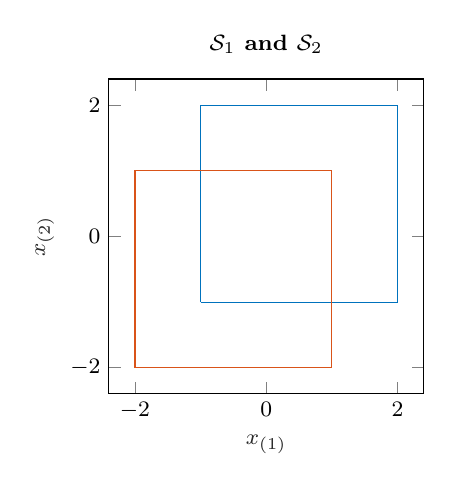
\begin{tikzpicture}
\footnotesize

\begin{axis}[%
width=4cm,
height=4cm,
at={(0in,0in)},
scale only axis,
xmin=-2.4,
xmax=2.4,
xlabel style={font=\color{white!15!black}},
xlabel={$x_{(1)}$},
ymin=-2.4,
ymax=2.4,
ylabel style={font=\color{white!15!black}},
ylabel={$x_{(2)}$},
axis background/.style={fill=white},
title style={font=\bfseries},
title={$\mathcal{S}_1$ and $\mathcal{S}_2$}
]
\addplot [color=mycolor1, forget plot]
  table[row sep=crcr]{%
-1	-1\\
2	-1\\
2	2\\
-1	2\\
-1	-1\\
};
\addplot [color=mycolor2, forget plot]
  table[row sep=crcr]{%
-2	-2\\
1	-2\\
1	1\\
-2	1\\
-2	-2\\
};
\end{axis}
\end{tikzpicture}%
\end{minipage}
\begin{minipage}[t]{0.2\textwidth}
	\vspace{10pt}

	\begin{verbatim}
	Command Window:
		
	res = true
	\end{verbatim}
\end{minipage}
\begin{minipage}[t]{0.3\textwidth}
	\vspace{0pt}
	\centering
	\includetikz{./figures/tikz/set-predicates/example_isIntersecting}
\end{minipage}
\end{center}

\begin{table}[htb]
	\centering
	\footnotesize
	\caption{Intersection checks implemented by the function \operator{isIntersecting}($\mathcal{S}_1,\mathcal{S}_2$) in CORA. The shortcuts e (exact check) and o (over-approximation) are used. If both, an exact and an over-approximative algorithm are implemented, we write e/o.}
	\label{tab:isIntersecting}
	\begin{tabular}{ l c c c c c c c c c c c c c}
		\toprule
					 & \textbf{I} & \textbf{Z} & \textbf{P} & \textbf{cZ} & \textbf{zB} & \textbf{E} & \textbf{C} & \textbf{tay} & \textbf{pZ} & \textbf{cPZ} & \textbf{hs} & \textbf{cHp} & \textbf{ls} \\
		\midrule
		\textbf{interval} (I)       		  & e   & e/o & e/o & e/o & e/o & o & o & o & o & o & e & e/o & o\\
		\textbf{zonotope} (Z)      		      & e/o & e/o & e/o & e/o & e/o & o & o & o & o & o & e & e/o & o\\
		\textbf{polytope} (P)   	          & e/o & e/o & e   & e/o & e/o & o & o & o & o & o & e & e/o & o\\
		\textbf{conZonotope} (cZ)		      & e/o & e/o & e/o & e/o & e/o & o & o & o & o & o & e & e/o & o\\
		\textbf{zonoBundle} (zB)  	      	  & e/o & e/o & e/o & e/o & e/o & o & o & o & o & o & e & e/o & o\\
		\textbf{ellipsoid} (E)       	      & o   & o   & o   & o   & o   & e & o & o & o & o & e & o & o\\
		\textbf{capsule} (C)				  & o   & o   & o   & o   & o   & o & e & o & o & o & e & o & o\\
		\textbf{taylm} (tay)    	          & o   & o   & o   & o   & o   &   &   &   & o & o & o & o & o\\
		\textbf{polyZonotope} (pZ)		      & o   & o   & o   & o   & o   &   &   & o & o & o & o & o & o\\
		\textbf{conPolyZono} (cPZ)		      & o   & o   & o   & o   & o   & o & o & o & o & o & o & o & o\\
		\textbf{levelSet} (ls)		  		  & o   & o   & o   & o   & o   & o & o & o & o & o &   &  & \\
		\bottomrule
	\end{tabular}
\end{table}



\subsubsubsection{isFullDim}

The method \operator{isFullDim} checks if a set is full-dimensional, that is, if the dimension of its affine hull is equal to the dimension of its ambient space. Given a set $\mathcal{S} \subset \Rn$, the method \operator{isFullDim} is defined as
	\begin{equation*}
		\operator{isFullDim}(\mathcal{S}) =
		\begin{cases}
			\operator{true}, & \exists x \in \mathcal{S}, \epsilon > 0: ~ x + \epsilon \mathcal{B} \subseteq \mathcal{S}, \\
			\operator{false} & \mathrm{otherwise,}
		\end{cases}
	\end{equation*}	
where $\mathcal{B} = \{x ~|~ ||x||_2 \leq 1 \} \subset \mathbb{R}^n$ is the unit ball. Let us demonstrate the method $\operator{isFullDim}$ by an example:

\begin{center}
\begin{minipage}[t]{0.40\textwidth}
	\vspace{10pt}
	\footnotesize
	% This file was automatically created from the m-file 
% "m2tex.m" written by USL. 
% The fontencoding in this file is UTF-8. 
%  
% You will need to include the following two packages in 
% your LaTeX-Main-File. 
%  
% \usepackage{color} 
% \usepackage{fancyvrb} 
%  
% It is advised to use the following option for Inputenc 
% \usepackage[utf8]{inputenc} 
%  
  
% definition of matlab colors: 
\definecolor{mblue}{rgb}{0,0,1} 
\definecolor{mgreen}{rgb}{0.13333,0.5451,0.13333} 
\definecolor{mred}{rgb}{0.62745,0.12549,0.94118} 
\definecolor{mgrey}{rgb}{0.5,0.5,0.5} 
\definecolor{mdarkgrey}{rgb}{0.25,0.25,0.25} 
  
\DefineShortVerb[fontfamily=courier,fontseries=m]{\$} 
\DefineShortVerb[fontfamily=courier,fontseries=b]{\#} 
  
\noindent       
 $$\color{mgreen}$% sets S1 and S2$\color{black}$$\\
 $S1 = zonotope([1 2 1;3 1 2]);$\\
 $S2 = zonotope([1 2 1;3 4 2]);$\\
 $$\\
 $$\color{mgreen}$% check if full-dimensional$\color{black}$$\\
 $res = isFullDim(S1)$\\
 $res = isFullDim(S2)$\\ 
  
\UndefineShortVerb{\$} 
\UndefineShortVerb{\#}
\end{minipage}
\begin{minipage}[t]{0.25\textwidth}
	\vspace{10pt}

	\begin{verbatim}	
	Command Window:
	
	res = true
	
	res = false
	\end{verbatim}
\end{minipage}
\end{center}




\subsubsubsection{isequal}

The method \operator{isequal} checks if two sets are identical. Optionally, a tolerance can be set to reduce the effect of floating-point deviations. Given two sets $\mathcal{S}_1,\mathcal{S}_2 \subset \Rn$, the method \operator{isequal} is defined as
	\begin{equation*}
		\operator{isequal}(\mathcal{S}_1,\mathcal{S}_2,\operator{tol}) =
		\begin{cases}
			\operator{true}, & \mathcal{S}_1 = \mathcal{S}_2 \\
			\operator{false} & \mathrm{otherwise}.
		\end{cases}
	\end{equation*}	
Let us demonstrate the method $\operator{isequal}$ by an example:

\begin{center}
\begin{minipage}[t]{0.40\textwidth}
	\vspace{10pt}
	\footnotesize
	\input{./MATLABcode/example_isequal}
\end{minipage}
\begin{minipage}[t]{0.25\textwidth}
	\vspace{10pt}

	\begin{verbatim}	
	Command Window:
	
	res = true
	\end{verbatim}
\end{minipage}
\end{center}

\vspace{1cm}

\subsubsubsection{representsa} \label{sec:representsa}

The method \operator{representsa} checks if a set can equivalently be represented by a different set, e.g. a special case.
Given a set $\mathcal{S} \subset \Rn$ and a string \operator{type}, the method \operator{representsa} is defined as
	\begin{equation*}
		\operator{representsa}(\mathcal{S},\operator{type},\operator{tol}) =
		\begin{cases}
			\operator{true}, & \mathcal{S} \text{ can be represented by } \operator{type}, \\
			\operator{false} & \mathrm{otherwise},
		\end{cases}
	\end{equation*}
where \operator{type} is the class name of another set representation or a special case, e.g. \operator{'point'}.
Let us demonstrate the method \operator{representsa} by an example to check if a given set is empty:

\begin{center}
\begin{minipage}[t]{0.40\textwidth}
	\vspace{10pt}
	\footnotesize
	% This file was created by matlab2tikz.
%
\definecolor{mycolor1}{rgb}{0.00000,0.44700,0.74100}%
\definecolor{mycolor2}{rgb}{0.85000,0.32500,0.09800}%
%
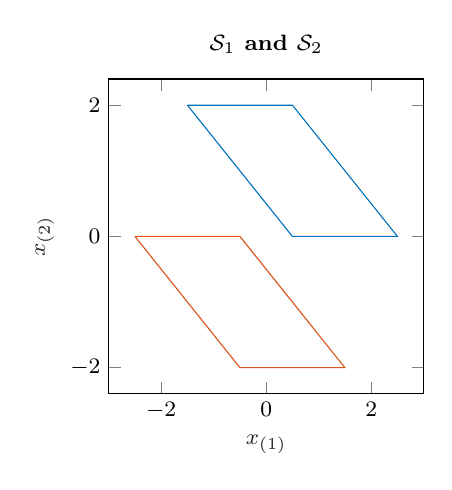
\begin{tikzpicture}
\footnotesize

\begin{axis}[%
width=4cm,
height=4cm,
at={(0in,0in)},
scale only axis,
xmin=-3,
xmax=3,
xlabel style={font=\color{white!15!black}},
xlabel={$x_{(1)}$},
ymin=-2.4,
ymax=2.4,
ylabel style={font=\color{white!15!black}},
ylabel={$x_{(2)}$},
axis background/.style={fill=white},
title style={font=\bfseries},
title={$\mathcal{S}_1$ and $\mathcal{S}_2$}
]
\addplot [color=mycolor1, forget plot]
  table[row sep=crcr]{%
-1.5	2\\
0.5	0\\
2.5	0\\
0.5	2\\
-1.5	2\\
};
\addplot [color=mycolor2, forget plot]
  table[row sep=crcr]{%
-2.5	0\\
-0.5	-2\\
1.5	-2\\
-0.5	0\\
-2.5	0\\
};
\end{axis}
\end{tikzpicture}%
\end{minipage}
\begin{minipage}[t]{0.2\textwidth}
	\vspace{10pt}

	\begin{verbatim}
	Command Window:
		
	res = true
	\end{verbatim}
\end{minipage}
\begin{minipage}[t]{0.3\textwidth}
	\vspace{0pt}
	\centering
	\includetikz{./figures/tikz/set-predicates/example_isempty}
\end{minipage}
\end{center}

Note: This function replaces the function \operator{isempty}.
The main reason is that \operator{isempty} is also called implicitly by MATLAB in various circumstances.
For example, \operator{isempty} is called on each workspace variable at a breakpoint,
which can lead to long loading times if the empty check is expensive for a given set representation.

